
%\chapter{Week2}

\section{Friday}\index{week2_Friday_lecture}
\subsection{symmetric matrix}
\begin{definition}[symmetric matrix]
A $n\x n$ matrix $\bm A$ is a \emph{symmetric matrix} if we have $\bm A\trans = \bm A$, which means $a_{ij}=a_{ji}$ for all $i,j$.
\end{definition}
For example, the matrix $\bm A$ shown below is a symmetric matrix:
\[
\begin{array}{ll}
\mbox{\emph{symmetric matrix}}
&
\bm A = \begin{bmatrix}
2&1\\1&3
\end{bmatrix}=\bm A\trans
\end{array}
\]
\begin{definition}[skew-symmetric matrix]
A $n\x n$ matrix $\bm A$ is a \emph{skew-symmetric matrix} or say, \emph{anti-symmetric matrix} if we have $\bm A = -\bm A\trans$.
\end{definition}
For example, matrix $\bm B$ shown below is a skew-symmetric matrix:
\[
\begin{array}{ll}
\mbox{\emph{skew-symmetric matrix}}
&
\bm B = \begin{bmatrix}
0&-1\\1&0
\end{bmatrix}=-\bm B\trans
\end{array}
\]
\begin{theorem}
Any $n\x n$ matrix can be decomposed as the sum of a \textit{symmetric} and a \textit{skew-symmetric} matrix.
\end{theorem}
\begin{proof}[Proofoutline.]
Given any $n\x n$ matrix $\bm A$, we can write $\bm A$ as:
\[
\bm A = \underbrace{\frac{\bm A+\bm A\trans}{2}}_{\mbox{symmetric}} + \underbrace{\frac{\bm A-\bm A\trans}{2}}_{\mbox{skew-symmetric}}
\]
\end{proof}
\newpage
\subsection{Interaction of inverse and transpose}
\begin{proposition}
If $\bm A$ exists, then $\bm A\trans$ also exists, and $(\bm A\trans)^{-1} = (\bm A^{-1})\trans$.
\end{proposition}
\begin{proof}
\[(\bm A^{-1}\bm A)\trans = \bm A\trans(\bm A^{-1})\trans = \bm I \implies (\bm A^{-1})\trans = (\bm A\trans)^{-1}\]
\end{proof}
\begin{corollary}
If matrix $\bm A$ is symmetric and invertible, then $\bm A^{-1}$ remains symmetric.
\end{corollary}
\begin{proof}
\[
(\bm A^{-1})\trans = (\bm A\trans)^{-1} = \bm A^{-1}
\implies \text{$\bm A^{-1}$ is symmetric.}
\]
\end{proof}
\begin{proposition}
If $\bm M = \begin{bmatrix}
\bm A&\bm B\\\bm C&\bm D
\end{bmatrix}$, then $\bm M\trans = \begin{bmatrix}
\bm A\trans&\bm C\trans\\\bm B\trans&\bm D\trans
\end{bmatrix}.$
\end{proposition}
\begin{corollary}
Given matrix $\bm M = \begin{bmatrix}
\bm A&\bm B\\\bm C&\bm D
\end{bmatrix}$, matrix $\bm M$ is symmetric if and only if \[
\bm A=\bm A\trans,\bm D =\bm D\trans,\bm B\trans = \bm C.
\]
\end{corollary}
\begin{proposition}
Suppose $\bm A$ is invertible and symmetric. When we do LDU decomposition such that $\bm A = \bm L\bm D\bm U$, $\bm U$ is exactly $\bm L\trans$.
\end{proposition}
\begin{proof}[Proofoutline.]
Note that
\[
\bm A\trans = (\bm{LDU})\trans = \bm U\trans\bm D\trans\bm L\trans=\bm A = \bm{LDU}.
\]

Since $\bm D$ is diagonal matrix, we have $\bm D = \bm D\trans$. It follows that
\[
\bm U\trans\bm D\bm L\trans= \bm{LDU}=\bm A.
\]

Since $\bm U\trans$ is also a lower triangular matrix, $\bm L\trans$ is also an upper triangular matrix, $\bm U\trans\bm D\bm L\trans$ is also the LDU decomposition of $\bm A$.

Due to the uniqueness of LDU decomposition, we obtain $\bm U\trans = \bm L,\bm L\trans = \bm U$.
\end{proof}
\subsection{Vector Space}
We move to a new topic: vector spaces. 
\paragraph{From Numbers to Vectors} We know matrix calculation(such as $\bm Ax = \bm b$) involves many numbers, but they are just linear combinations of $n$ vectors.  
\paragraph{Third Level Undetstanding} This topic moves from numbers and vectors to a third level of understanding (the highest level). Instead of individual column vectos, we look at  "\textit{spaces}" of vectors. And this topic will end with the "\textit{Fundamental Theorem of Linear Algebra}".
\[\begin{array}{ll}
\mbox{Matrix Calculation: }
&
\mbox{Numbers}\implies
\mbox{Vectos}
\implies
\mbox{\emph{Spaces}}
\end{array}
\]
We begin with the typical vector space, which is denoted as $\mathbb{R}^{n}$.
\begin{definition}[Real Space]
The space $\mathbb{R}^{n}$ contains all column vectors $v$ such that $v$ has $n$ real number entries.
\end{definition}
\paragraph{Notation} We denote vectors as \textit{a
column between brackets}, or \textit{along a line using commas and parentheses:}
\[
\begin{array}{ll}
\begin{bmatrix}
4\\\pi
\end{bmatrix}
\mbox{ is in $\mathbb{R}^{2}$}
&
(1,1,1)
\mbox{ is in $\mathbb{R}^{3}.$}
\end{array}
\]
\begin{definition}[vector space]
A \emph{vector space} $\bm V$ is a set of vectors such that these vectors satisfy \textit{vector addition} and \textit{scalar multiplication}:
\begin{itemize}
\item
\emph{vector addition:}If vector $v$ and $w$ is in $\bm V$, then $v+w\in \bm V.$
\item
\emph{scalar multiplication:}If vector $v\in \bm V$, then $cv\in \bm V$ for any real numbers $c$.
\end{itemize}
\end{definition}
In other words, the set of vectors is \emph{closed} under \textit{addition} $v + w$ and \textit{multiplication} $cv$. In other words, 
\begin{quotation}
\emph{any linear combination is closed under vector space.}
\end{quotation}
\begin{proposition}
Every vector space must contain the zero vector.
\end{proposition}
\begin{proof}
Given $v\in\bm V\implies -v\in\bm V\implies v+(-v) = \bm 0\in \bm V.$
\end{proof}
\begin{example}
\[
\bm V = \left\{\begin{pmatrix}
a_1\\a_2\\\vdots\\a_n\\\vdots
\end{pmatrix}
\middle|
 \{a_n\}\text{ is infinite length sequences.} \right\}
\] 
is a vector space.

This is because for any vector $v = \begin{pmatrix}
a_1\\a_2\\\vdots\\a_n\\\vdots
\end{pmatrix},w = \begin{pmatrix}
b_1\\b_2\\\vdots\\b_n\\\vdots
\end{pmatrix}$, we can define vector addition and scalar multiplication as follows:
\[
\begin{array}{ll}
v+w = \begin{pmatrix}
a_1+b_1\\a_2+b_2\\\vdots\\a_n+b_n\\\vdots
\end{pmatrix}
&
cv = \begin{pmatrix}
ca_1\\ca_2\\\vdots\\ca_n\\\vdots
\end{pmatrix}
\mbox{ for any $c\in\mathbb{R}$}.
\end{array}
\]
\[
\begin{aligned}
\bm V &= \Span\left\{v_1=\begin{pmatrix}
\frac{1}{2}\\\frac{1}{4}\\\vdots\\\frac{1}{2^n}\\\vdots
\end{pmatrix},v_2=\begin{pmatrix}
\frac{1}{3}\\\frac{1}{9}\\\vdots\\\frac{1}{3^n}\\\vdots
\end{pmatrix},v_3=\begin{pmatrix}
\frac{1}{4}\\\frac{1}{16}\\\vdots\\\frac{1}{4^n}\\\vdots
\end{pmatrix}\right\} \\
&= \{\alpha_1v_1+\alpha_2v_2+\alpha_3v_3\mid \alpha_1,\alpha_2,\alpha_3\in\mathbb{R}\}
\end{aligned}
\] 
is also vector space. 

\begin{definition}[Span]
The \emph{span} of a collection of vectors $\bm a_1,\dots,\bm a_n\in\mathbb{R}^m$ is defined as:
\[
\Span\{\bm a_1,\dots,\bm a_n\}
=\left\{
\bm y\in\mathbb{R}^m\middle|\bm y=\sum_{i=1}^n\alpha_i\bm a_i, \bm\alpha\in\mathbb{R}^n
\right\},
\]
i.e., it is the set of all linear combinations of $\bm a_1,\dots,\bm a_n$.
\end{definition}

How to check $\bm V$ is a vector space?

Given any two vectors $u,w$ in $\bm V$, suppose 
\[
\begin{array}{ll}
u = \alpha_1v_1+\alpha_2v_2+\alpha_3v_3,
&
v=\beta_1v_1+\beta_2v_2+\beta_3v_3,
\end{array} 
\] 
then we obtain:
\[
\begin{split}
\gamma_1u+\gamma_2v &= \gamma_1(\alpha_1v_1+\alpha_2v_2+\alpha_3v_3)+\gamma_2(\beta_1v_1+\beta_2v_2+\beta_3v_3) \\&= (\gamma_1\alpha_1+\gamma_2\beta_1)v_1+(\gamma_1\alpha_2+\gamma_2\beta_2)v_2+(\gamma_1\alpha_3+\gamma_2\beta_3)v_3
\end{split}
\]
where $\gamma_1,\gamma_2\in\mathbb{R}$. Hence any linear combination of $u$ and $w$ are also in $\bm V$. Hence $\bm V$ is a vector space.
\end{example}
\begin{example}
$\bm F = \{f(x) \mid f:[0,1]\mapsto \mathbb{R}\}$ is also a vector space. (verify it by yourself.) 

This vector space $\bm F$ contains all real functions defined on $[0,1]$, an it is infinite dimensional. 

Given two functions $f$ and $g$ in $\bm F$, the inner product of $f$ and $g$ is defined as:
\[
\inp{f}{g} := \int_0^1f(x)g(x)\diff x
\]
Also, we can use the span to form a vector space:
\[
\bm F = \Span\{sinx,x^3,e^x\} = \{\alpha_1sinx+\alpha_2x^3+\alpha_3e^x\mid \alpha_1,\alpha_2,\alpha_3\in\mathbb{R}.\}
\]
This set $\bm F$ is also a vector space.
\end{example}
\begin{example}
\[
\bm V = \left\{\begin{bmatrix}
a_{11}&a_{12}&a_{13}\\a_{21}&a_{22}&a_{23}
\end{bmatrix}\middle| a_{ij}\in\mathbb{R}\text{ for $i=1,2; j=1,2,3.$}\right\}
\] 
is a vector space. Moreover, it is equivalent to the span of six basic vectors:
\[
\bm V = \Span\left\{
\begin{bmatrix}
1&0&0\\0&0&0
\end{bmatrix},\begin{bmatrix}
0&1&0\\0&0&0
\end{bmatrix},\begin{bmatrix}
0&0&1\\0&0&0
\end{bmatrix},\begin{bmatrix}
0&0&0\\1&0&0
\end{bmatrix},\begin{bmatrix}
0&0&0\\0&1&0
\end{bmatrix},\begin{bmatrix}
0&0&0\\0&0&1
\end{bmatrix}
\right\}
\]
We say that $\bm V$ is 6-dimensional without introducing the definiton of dimension formally.
\end{example}
\begin{example}
\[
\bm V = \left\{\begin{bmatrix}
a_{ij}
\end{bmatrix}_{3\x 3}\middle| \text{any $3\x 3$ matrices}\right\}
\]
 is also a vector space.
 
Obviously, it is 9-dimensional. We usually denote it as $\dim(\bm V) = 9$.

\[\bm V_1 = \left\{\begin{bmatrix}
a_{ij}
\end{bmatrix}_{3\x 3}\middle| \text{any $3\x 3$ symmetric matrices}\right\}
\] 
is a special vector space.

Notice that $\bm V_1\subset\bm V$, so we say $\bm V_1$ is a \textit{subspace} of $\bm V$. In the future we will know $\dim(\bm V_1) = 6<9$.
\end{example}
\subsubsection{The solution to $\bm{Ax}= \bm 0$}
We can use vector space to discuss the solution to system of equation. Firstly, let's introduce some definitions:
\begin{definition}[homogeneous equations]
A system of linear equations is said to be \emph{homogeneous} if the constants on the righthand
side are all zero. In other words, $\bm{Ax} = \bm 0$ is said to be \emph{homogeneous}.
\end{definition}
\begin{definition}[column space]
The column space consists of all linear combinations of the columns of matrix $\bm A$. In other words, for the matrix $\bm A\in\mathbb{R}^{m\times n}$ given by $\bm A = \left[
\begin{array}{c|c|c|c}
a_1&a_2&\ldots&a_n
\end{array}\right]$, its column space is denoted as 
\[
\bm C(\bm A) := \Span(a_1,a_2,\dots,a_n)\subset\mathbb{R}^{m}.
\]
\end{definition}
\begin{definition}[null space]
The null space of a matrix $\bm A\in\mathbb{R}^{m\times n}$ consists of all solutions to $\bm{Ax} = \bm 0$, which can be denoted as 
\[
\bm N(\bm A) = \{\bm x\mid\bm{Ax} = \bm 0\}\subset\mathbb{R}^{n}.
\]
\end{definition}
\begin{proposition}
The null space $\bm N(\bm A)$ is a vector space.
\end{proposition}
\begin{proof}[Proofoutline.]
For any two vectors $\bm x,\bm y\in\bm N(\bm A)$, we have $\bm{Ax} = \bm 0,\bm{Ay} = \bm 0$.
\[
\begin{array}{ll}
\implies \bm A(\alpha\bm x +\beta\bm y) = \alpha(\bm{Ax})+\beta(\bm{Ay}) = \alpha\bm 0+\beta\bm 0 = \bm 0
&
\alpha,\beta\in\mathbb{R}.
\end{array}
\]
Since the linear combination of $\bm x$ and $\bm y$ is also in $\bm N(\bm A)$, $\bm N(\bm A)$ is a vector space.
\end{proof}
\begin{example}
Describe the null space of $\bm A = \begin{bmatrix}
1&0\\5&0\\2&3
\end{bmatrix}.$\\
Obviously, converting matrix into linear system of equation we obtain:
\[
\left\{\begin{lgathered}
x_1+0x_2=0\\5x_1+4x_2=0\\2x_1+3x_2=0
\end{lgathered}\right.
\]
We can easily obtain the solution 
$\left\{\begin{lgathered}
x_1=0\\x_2=0
\end{lgathered}\right.$. 
Hence the null space is $\bm N(\bm A) = \bm 0$.
\end{example}
\begin{example}
Describe the null space of $\bm A = \begin{bmatrix}
1&0&1\\5&4&9\\2&3&5
\end{bmatrix}.$

In the next lecture we will know its null space is a line.

We find that $\bm A\begin{pmatrix}
1\\1\\-1
\end{pmatrix}= \bm 0$, so $\begin{pmatrix}
1\\1\\-1
\end{pmatrix}$ is a special solution. 

Note that \textit{the null space contains all linear combinations of special solutions.} Hence the null space is $\bm N(\bm A) = \left\{c\begin{pmatrix}
1\\1\\-1
\end{pmatrix}\middle| c\in\mathbb{R}\right\}$.
\end{example}
\subsubsection{The complete solution to $\bm{Ax} = \bm b$}
In order to find all solutions of $\bm{Ax} = \bm b$, ($\bm A$ may not be square matrix), let's introduce two kinds of solutions:

\begin{definition}[Particular $\&$ Special Solution]
For the system of equations $\bm A\bm x=\bm b$, there are two kinds of solutions:
\[
\begin{array}{ll}
\bm{x_{\mbox{particular}}}
&
\mbox{\emph{The particular solution that solves $\bm{Ax} = \bm b$}}
\end{array}
\]
\[
\begin{array}{ll}
\bm{x_{\mbox{nullspace}}}
&
\mbox{\emph{The special solutions that solves $\bm{Ax} = \bm 0$}}
\end{array}
\]
\end{definition}
There is a theorem that helps us to obtain the complete solution to $\bm{Ax} = \bm b$.
\begin{theorem}
Any solution to $\bm{Ax} = \bm b$ can be represented as $\bm{x_{complete}} = \bm{x_p} + \bm{x_n}$.
\end{theorem}
\begin{proof}
\begin{proof}[Sufficiency.]Given $\bm{x_{complete}} = \bm{x_p} + \bm{x_n}$, it suffices to show $\bm{x_{complete}}$ is the solution to $\bm{Ax} = \bm b$. 

Note that
\[
\bm A\bm{x_{complete}} = \bm A(\bm{x_p} + \bm{x_n}) = \bm A\bm{x_p}+\bm A\bm{x_n} = \bm b+\bm 0 = \bm b.
\]
Hence $\bm{x_{complete}}$ is the solution to $\bm{Ax} = \bm b$.
\end{proof}
\begin{proof}[Necessity.]Suppose $\bm x^*$ is the solution to $\bm{Ax} = \bm b$, it suffices to show $\bm x^*$ could be represented as $\bm{x_p} + \bm{x_n}$. 

It suffices to show $\bm x^*- \bm{x_p}\in \bm N(\bm A)$.

Notice that $\bm A(\bm x^*-\bm{x_p}) = \bm A\bm x^*-\bm A\bm{x_p} = \bm b-\bm b = \bm 0\implies \bm x^*- \bm{x_p}\in \bm N(\bm A)$. 
\end{proof}\end{proof}
\begin{example}
Let's study a system that has $n=2$ unknowns but only $m=1$ equation:
\[
x_1+x_2 = 2.
\]
It's easy to check that the particular solution is $\bm{x_p} = \begin{pmatrix}
1\\1
\end{pmatrix}$, the special solutions are $\bm{x_n} = c\begin{pmatrix}
1\\-1
\end{pmatrix}$, $c$ can be taken arbitararily.

Hence the complete solution for the equations could be written as 
\[\bm{x_{complete}} = \bm{x_p}+\bm{x_n} = \begin{pmatrix}
c+1\\-c+1
\end{pmatrix}.\]

So we summarize that if there are $n$ unknowns and $m$ equations such that $m<n$, then $\bm{Ax} = \bm b$ is \emph{underdetermined} (It may have infinitely many solutions since the special solutions could be infinite).
\begin{figure}[H]
\centering
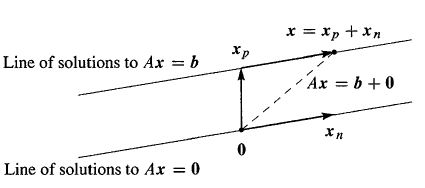
\includegraphics{week2/complete.jpg}
\caption{Complete solution = one particular solution + all nullspace solutions}
\end{figure}
\end{example}
\subsubsection{Row-Echelon Matrices}
Given $m\x n$ rectangular matrix $\bm A$, we can still do Gaussian Elimination to convert $\bm A$ into $\bm U$, where $\bm U$ is of \emph{Row Echelon form}. The whole process could be expressed as:
\[
\bm{PA} = \bm{LDU}.
\]
where $\bm L$ is $m\x m$ \emph{lower triangular} matrix, $\bm U$ is $m\x n$ matrix that is of \emph{row echelon form}.

\begin{example} Here is a $4\x 7$ row echelon matrix with the three pivots $\bm 1$ highlighted in blue:
\[
\bm U = \left[
\begin{array}{@{}ccccccc@{}}
\cellcolor{cyan!50}1&\x&\x&\x&\x&\x&\x\\
0&\cellcolor{cyan!50}1&\x&\x&\x&\x&\x\\
0&0&0&0&0&\cellcolor{cyan!50}1&\x\\
0&0&0&0&0&0&0
\end{array}
\right]
\]
\begin{itemize}
\item
Columns 3,4,5,7 have no pivots, and we say the free variables are $x_3,x_4,x_5,x_7.$
\item
Columns 1,2,6 have pivots, and we say the pivot variables are $x_1,x_2,x_6.$
\end{itemize}
Moreover, we can continue Gaussian Elimination to convert $\bm U$ into $\bm R$ that is of \emph{reduced row echelon form}:
\[
\bm R = \left[
\begin{array}{@{}ccccccc@{}}
\cellcolor{cyan!50}1&0&\x&\x&\x&0&\x\\
0&\cellcolor{cyan!50}1&\x&\x&\x&0&\x\\
0&0&0&0&0&\cellcolor{cyan!50}1&\x\\
0&0&0&0&0&0&0
\end{array}
\right]
\]
\emph{The reduced row echelon matrix $\bm R$ has zeros above the pivots as well as below. Zeros above the pivots come from upward elimination.}
\end{example}
\begin{remark}
Remember the two steps (forward and back elimination) in solving $\bm{Ax} = \bm b$:
\begin{enumerate}
\item
\emph{Forward Elimination} takes $\bm A$ to $\bm U$. (or its reduced form $\bm R$)
\item
\emph{Back Elimination} in $\bm{Ux} = \bm c$ or $\bm{Rx} = \bm d$ produces $\bm x$.
\end{enumerate}
\end{remark}

\subsubsection{Problem Size Analysis}
When faced with $m\x n$ matrix $\bm A$, notice that $\bm m$ refers to the \emph{number of equations}, $\bm n$ refers to the \emph{number of variables}. Assume $\bm r$ denotes \emph{number of pivots}, then we know $\bm r$ is also the \emph{number of pivot variables}, $\bm n-\bm r$ is the \emph{number of free variables}. Finally we have $\bm m-\bm r$ \emph{redundant equations} and $\bm r$ \emph{irredundant equations}. In next lecture, we will introduce the definition for $\bm r$ formally (rank).










